\documentclass{exam} 
%\documentclass[answers]{exam} 
\usepackage{amsmath,amssymb,enumitem,fdsymbol,float,tikz,pgfplots,etoolbox,ifthen,xcolor,fullpage,ulem,graphicx,comment,hyperref} 
\addpoints
\marksnotpoints
\usetikzlibrary{calc}
\usetikzlibrary{math} % for \tikzmath
\usetikzlibrary{angles,quotes}
\definecolor{MyGreen}{rgb}{0.1, 0.4, 0.1}
\AtBeginEnvironment{solution}{\color{MyGreen}}

%\printanswers (or \noprintanswers) to see the solutions (or not). \noprintanswers is the default so just comment/uncomment the next line:

\printanswers

%Add rubrics
\usepackage{tagging}
% Comment out this line to hide the rubric text:
\usetag{rubric}

\definecolor{MyBlue}{rgb}{0.1, 0.1, 0.9}

\newcommand\rubric[1]{\tagged{rubric}{\textcolor{MyBlue}{#1}}}

\newenvironment{rubricEnv}{\taggedblock{rubric} \color{MyBlue}}{\endtaggedblock}

\newcommand{\onestar}{\raisebox{0.05cm}{\resizebox{1.6cm}{!}{$\bigstar\largewhitestar\largewhitestar\largewhitestar$ \ }}}
\newcommand{\twostar}{\raisebox{0.05cm}{\resizebox{1.6cm}{!}{$\bigstar\bigstar\largewhitestar\largewhitestar$ \ }}}
\newcommand{\threestar}{\raisebox{0.05cm}{\resizebox{1.6cm}{!}{$\bigstar\bigstar\bigstar\largewhitestar$ \ }}}
\newcommand{\fourstar}{\raisebox{0.05cm}{\resizebox{1.6cm}{!}{$\bigstar\bigstar\bigstar\bigstar$ \ }}}

\newcommand\pts[1][2]{\text{\bf [#1 pts]}}
\newcommand\pt{\text{\bf [1 pt]}}

%\setlength\parindent{0in}
%\pagestyle{empty}

\everymath{\displaystyle}
\newcommand{\diff}[2]{\frac{\text{d}#1}{\text{d}#2}}

\newcommand\rightAngle[4]{
  \pgfmathanglebetweenpoints{\pgfpointanchor{#2}{center}}{\pgfpointanchor{#3}{center}}
  \coordinate (tmpRA) at ($(#2)+(\pgfmathresult+45:#4)$);
  %\draw[white,line width=0.6] ($(#2)!(tmpRA)!(#1)$) -- (tmpRA) -- ($(#2)!(tmpRA)!(#3)$);
  \draw[blue!40!black] ($(#2)!(tmpRA)!(#1)$) -- (tmpRA) -- ($(#2)!(tmpRA)!(#3)$);
}
\colorlet{myblue}{blue!70!black}
\colorlet{mygreen}{green!40!black}
\colorlet{myred}{red!65!black}
\begin{document}

\subsection*{ASSIGNMENT 3}

\subsubsection*{Learning goals}
\begin{itemize}
    \setlength\itemsep{0.1em}
    \item Extend your understanding of concavity to the concept of \textit{curvature}  for a curve given as the graph of a function $y=f(x)$. 
    \item Define and find the \textit{radius of curvature} at a given point on $y=f(x)$.
    \item Find the equation of the \textit{osculating circle}, which has the same tangent line as the curve $y=f(x)$ at a given point and shares the same curvature there. 
    \item Practice graphing functions.
\end{itemize}
\hrulefill

\subsubsection*{Contributors}

\textit{On the first page of your submission, list the student numbers and full names (with the last name in \textbf{bold}) of all team members. Indicate members who have not contributed using the comment ``(non-contributing)''.}

\noindent\hrulefill

\subsubsection*{Reflection question}

\textit{Reflection questions encourage you to think about how mathematics is done. This is an important ingredient of success. Reflection questions contribute to your \textbf{engagement grade}.}

\begin{questions}

\question At this point in the course, having written the first test and completed a pair of assignments, it is appropriate to take stock of your habits. The following simple survey generates an individual score.

\begin{itemize}
    \item \textit{For the past five weeks, I have done deliberate problem-solving practice for one hour a day, six days a week.}
    
    If this is true, give yourself 10 points. Otherwise, give yourself 0 points.

\item \textit{For the past five weeks, I have attended all small classes (except in cases of illness or emergency).}

    If this is true, give yourself 4 points. If you have missed one small class, give yourself 1 point. Otherwise, give yourself 0 points.
    
\item \textit{For the past five weeks, I have attended all lectures (except in cases of illness or emergency).}

    If this is true, give yourself 3 points. If you have missed one lecture, give yourself 1 point. Otherwise, give yourself 0 points.

\item \textit{For the past five weeks, I have started all assignments at least 5 days before the due date.}

    If this is true, give yourself 3 points. If it is true in all but one case, give yourself 1 point. Otherwise, give yourself 0 points.
    
\end{itemize}

What is the average score of your team members? (Be honest with yourselves; no points will be awarded based on what this average score is.) In one or two paragraphs, describe at least two concrete steps you can take to help each other raise that score.

    \begin{solution}
        Put your solution here.
    \end{solution}

\end{questions}


\noindent\hrulefill


\subsubsection*{Assignment questions}



\textit{The questions in this section contribute to your \textbf{assignment grade}. Stars indicate the difficulty of the questions, as described on Canvas.}

\


In this assignment, you will explore the notion of \textit{curvature} through a classical differential geometric quantity $\kappa$ that measures how much a curve deviates from being a straight line. We will be interested in the particular case of curves that are graphs of functions $y=f(x)$, where the function $f(x)$ is \textit{twice-differentiable}, meaning $f'(x)$ and $f''(x)$ exist.  In this case, $\kappa$ will be a function of $x$, $\kappa(x)$.

\

The circle will form the basis for our thinking about curvature; we want its curvature to be the same at every point on the circle. Let us define \textit{the curvature at any point on a circle} to be $\kappa = 1/R$, where $R$ is the radius of the circle. Note the smaller the radius of the circle, the larger its curvature, and the larger the radius of the circle, the smaller its curvature.

\

Since we intend to define curvature for more general curves by studying the way the curve deviates from its tangent line at any point, we expect the curvature of a straight line to be 0. For now, let us define \textit{the curvature of a straight line} to be 0. 


\begin{figure}[h]
\begin{center}
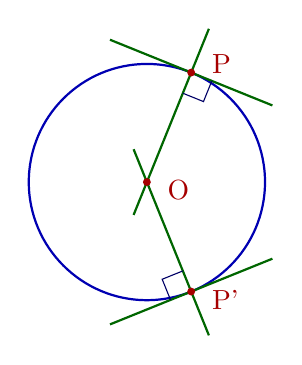
\begin{tikzpicture}
  \def\r{1.5} % radius
  \def\q{4} % distance center-external point q = |OQ|
  \def\x{{\r^2/\q}} % Q x coordinate
  \def\y{{\r*sqrt(1-(\r/\q)^2}} % Q y coordinate
  \coordinate (O) at (0,0); % circle center O
  \coordinate (Q) at (\q,0); % external point Q
  \coordinate (P) at (\x,\y); % point of tangency, P
  \coordinate (P') at (\x,-\y);
  %\draw[->] (0,-1.3*\r) -- (0,1.5*\r);
  %\draw[->] (-1.3*\r,0) -- (\q+0.4*\r,0);
  %\draw[dashed] (\x,0) |- (0,\y);
  \draw[myblue,thick] (O) circle(\r);
  \draw[mygreen,thick] ($(Q)!+0.7!(P)$) -- ($(Q)!1.3!(P)$);
  \draw[mygreen,thick] ($(Q)!+0.7!(P')$) -- ($(Q)!1.3!(P')$);
  \draw[mygreen,thick] ($(O)!-0.3!(P)$) -- ($(O)!1.4!(P)$);
  \draw[mygreen,thick] ($(O)!-0.3!(P')$) -- ($(O)!1.4!(P')$);
  \rightAngle{Q}{P}{O}{0.40}
  \rightAngle{Q}{P'}{O}{0.40}
  \fill[myred] (O) circle(0.05) node[below=3, right=4] {O};
 % \fill[myred] (Q) circle(0.05) node[below left] {Q};
  \fill[myred] (P) circle(0.05) node[above=3,right=4] {P};
  \fill[myred] (P') circle(0.05) node[below=3,right=4] {P'};
  
\end{tikzpicture}
\caption{The symmetry of a circle means the circle deviates from its tangent line at point $P$ in the same way as at point $P'$ for any pair of points $P$ and $P'$.}
\end{center}
\end{figure}

Consider now curves that are the graphs of functions $y=f(x)$, where $f(x)$ is a \textit{twice-differentiable function} -- both $f'(x)$ and $f''(x)$ exist. We can consider such curves to be \textit{smooth} in the sense there is a tangent line at every point on the curve, and the concavity is also defined at every point. 

\

Since we suppose $f''(x)$ exists everywhere, we are able to use it to study the way the slopes of tangent lines change nearby any point on the curve -- if $f''(x)$ is large at any point, then the slopes of tangent lines undergo a large change as we move through that point. This means the graph of the function near such a point has a very sharp turn in it. 

\

We will define the \textit{curvature} of a curve given by $y=f(x)$ to be 
$$
\kappa(x) = \frac{|f''(x)|}{\left(1+(f'(x))^2\right)^{3/2}}.
$$
Now that we have a value for the curvature of a function at a given point, we can define the \textit{radius of curvature} at that point to be \[\rho(x)=\frac{1}{\kappa(x)},\] whenever $\kappa(x)\neq 0.$ We can associate to $\rho(x)$ a circle of this radius tangent to the curve $y=f(x)$ at the point $(x,y)$.  This circle is the circle that best approximates the curvature of the curve at this point, and the graph of the function and this circle have the same tangent line at this point. This circle is called the \textit{osculating circle}.

\begin{questions}\setcounter{question}{1}

\question \onestar Show that $\kappa(x)=0$ for any straight line $y=f(x)=mx+b$.


    \begin{solution}
    
    Since $m$ and $b$ are constants, the first ans second derivatives of $f(x)$ are thus:
   	\begin{align*}
   	f'(x) &= m \\
   	f''(x) &= 0
   	\end{align*}
   	Now, since we know that the function $\kappa$ is a fraction with $|f''(x)|$ in the numerator, if $f''(x) = 0$, then $\kappa(x) = 0$ for all values of $x$. 
    
    \end{solution}

    

\question \threestar Consider the parabola $y=x^2$.
\begin{parts} 
    \part Find the curvature $\kappa(x)$ for this parabola and plot this curvature function. Identify the value of $x$ where $\kappa(x)$ is largest. 

    
    \begin{solution}
        
    We can begin by writing $y$ as a function of $x$ as $f(x) = x^2$.
    Now, we can take the first and second derivatives of $f(x)$:
    \begin{align*}
    f'(x) &= 2x\\
    f''(x) &= 2
    \end{align*}
    Now, given our first and second derivatives $f'(x)$ and $f''(X)$, we plug these functions into $\kappa(x)$ to get get the curvature function of this parabola $f(x) = x^2$:
    \begin{align*}
	\kappa(x) &= \frac{|f''(x)|}{\left(1+(f'(x))^2\right)^{3/2}}\\
	\kappa(x) &= \frac{|2|}{\left(1+(2x)^2\right)^{3/2}}\\
	\kappa(x) &= \frac{2}{(4x^2+1)^{3/2}}
    \end{align*}
    To find the value of $x$ where $\kappa(x)$ is largest, we should first take the derivative of $\kappa$ in order to find its critical point(s) where $\kappa'(x) = 0$:
    \begin{align*}
    \kappa'(x) &= -\frac{24x}{(1+4x^2)^{5/2}}\\
    0 &= -\frac{24x}{(1+4x^2)^{5/2}}\\
    x &= 0
    \end{align*}
    Since there is only one critical point, we should find out whether the function is increasing or decreasing before and after the critical point. Since the interval $(-\infty , x)$ is necessarily a negative number, the numerator of the function will be negative but the denominator will remain positive because the $x$ term is squared. Therefore, the double negative within the function $\kappa'(x)$ when ${x|x<0}$ means that $\kappa(x)$ is increasing at $(-\infty , 0)$. Now, when $(0 , \infty)$, both numerator and denominator are positive, and the function by extension is negative. Therefore, we know that $\kappa(x)$ is decreasing at interval $(0 , \infty)$. If a function increases up until a critical point and decreases afterwards, and the critical point is a local maximum. Since it is the only local maximum, under these conditions it is also the global maximum. Therefore, $\kappa(x)$ is greatest when $x=0$.
    
    \end{solution}

    
    \part Find the radius of curvature $\rho(x)$, and plot this function. Identify the value of $x$ where $\rho(x)$ is smallest.

    
    \begin{solution}
    
    Put your solution here.
    
    \end{solution}
    

    
    \part Consider the value of $x$ where $\kappa(x)$ is largest. Find the equation of the osculating circle for the parabola $y=x^2$ at this point and plot this circle and the parabola $y=x^2$ on the same axes. Remember the general form of the equation of a circle is $(x-x_0)^2+(y-y_0)^2=r^2,$ where $(x_0,y_0)$ is the centre of the circle.
    
    
    \begin{solution}
        
    Put your solution here.
    
    \end{solution}

    
    \part What is the behaviour of $\kappa(x)$ for large positive and negative values of $x$?  What does this tell you about the radii of the osculating circles, asymptotically speaking, for this parabola for $x\to \pm\infty$?

    
    \begin{solution}
    
    Put your solution here.
    
    \end{solution}

    
\end{parts}

\question \threestar Consider the cubic $y=x^3$.
\begin{parts} 
    
    \part Find the curvature $\kappa(x)$ for this cubic and plot this curvature function. Identify the values of $x$ where $\kappa(x)$ is largest. 

    
    \begin{solution}
        
    Put your solution here.
    
    \end{solution}

    
    \part Find the radius of curvature $\rho(x)$, plot this function, and identify the values of $x$ where $\rho(x)$ is smallest.

    
    \begin{solution}
        
    Put your solution here.
    
    \end{solution}

    
    \part Consider the values of $x$ where $\kappa(x)$ is largest. Find the equations of the osculating circles for the cubic $y=x^3$ at these points, and plot these circles and the cubic $y=x^3$ on the same axes. Remember the general form of the equation of a circle is $(x-x_0)^2+(y-y_0)^2=r^2,$ where $(x_0,y_0)$ is the centre of the circle.
    
    
    \begin{solution}
        
    Put your solution here.
    
    \end{solution}

    
    \part What is the behaviour of $\kappa(x)$ for large positive and negative values of $x$?  What does this tell you about the radii of the osculating circles, asymptotically speaking, for this cubic for $x\to \pm\infty$?

    
    \begin{solution}
    
    Put your solution here.
    
    \end{solution}

    
\end{parts}

\question \fourstar Show the formula for $\kappa(x)$ yields $\kappa(x)=1/R$ for a circle of radius $R$. (Thus, we can conclude that the general formula we have for the curvature $\kappa(x)$ of a curve $y=f(x)$ is consistent with  our initial definition of curvature for a circle.)


    \begin{solution}
    
    Put your solution here.
    
    \end{solution}

    
\end{questions}





\
\noindent\hrulefill





\end{document}